\documentclass[11pt]{article}

\usepackage[margin=1in]{geometry}
\usepackage[T1]{fontenc}
% Libertine text/math when available.
\IfFileExists{libertine.sty}{%
  \usepackage{libertine}%
  \IfFileExists{newtxmath.sty}{\usepackage[libertine]{newtxmath}}{}%
}{}
% Light monospace for inline code.
\IfFileExists{inconsolata.sty}{\usepackage[scaled=0.95]{inconsolata}}{%
  \IfFileExists{zi4.sty}{\usepackage[varqu,scaled=0.95]{zi4}}{}}
\usepackage{booktabs}
\usepackage{graphicx}
\usepackage{amsmath}
\usepackage{array}
\usepackage[table]{xcolor}
\usepackage[hidelinks]{hyperref}
\usepackage{caption}

\captionsetup{font=small,labelfont=bf,skip=4pt}
\definecolor{hdrgray}{gray}{0.92}
\definecolor{keyrow}{RGB}{226,239,246}
\newcommand{\code}[1]{\texttt{#1}}
\newcommand{\best}[1]{\textbf{#1}}
\newcommand{\hdr}{\rowcolor{hdrgray}}
\newcommand{\key}{\rowcolor{keyrow}}
\setlength{\emergencystretch}{3em}

\newenvironment{ctab}{\par\medskip\centering\small
  \setlength{\tabcolsep}{5pt}\renewcommand{\arraystretch}{1.12}}{\par\medskip}

% Full-width abstract aligned with the body margins.
\renewenvironment{abstract}{%
  \par\medskip\noindent{\bfseries\abstractname.}\enspace\ignorespaces
}{\par\medskip}

\title{\textbf{MongoDB for PageIndex Retrieval:\\ Benchmark,
Diagnosis, and Deployment Plan}}
\author{Junyao Dong}
\date{}

\begin{document}
\maketitle

\begin{abstract}
PageIndex stores documents as large hierarchical JSON trees that an agent
navigates from the root to relevant nodes. This report benchmarks the exact
storage calls issued by ConDB's retrievers on MongoDB, PostgreSQL/JSONB, DuckDB,
and SQLite, at scales up to ten million nodes.
MongoDB is competitive on navigation reads, content fetch, writes, concurrency,
and storage footprint. The one operation that stresses it,
\code{get\_subtree}---a materialized-path range scan matching tens of thousands
of nodes---is a schema problem rather than an engine ceiling: MongoDB's unit of
read is the whole document, and a non-covered scan performs one \code{FETCH} per
matched node, a behavior MongoDB's product team confirmed and that newer server
versions do not change. ConDB's deployed schema therefore decouples the tree:
node structure in one collection, per-node metadata in a key-value collection
keyed by node id, and leaf text in a third. Under this schema the subtree scan
is served index-only from the structure collection with zero document fetches,
and \code{get\_subtree} on the ten-million-node tree lands at $11.9$\,ms P50 /
$130$\,ms P95, within ${\sim}1.4{\times}$ of PostgreSQL at both the median and
the tail. The deployment plan follows the same design: ship the decoupled
schema, lead indexes and shard keys with \code{tree\_id}, keep the lean covering
index on the structure collection, and reserve subtree denormalization for
measured bottlenecks.
\end{abstract}

\section{Introduction}

ConDB indexes a document as a PageIndex tree: a hierarchy of nodes carrying a
title, a summary, page indices, and (at the leaves) text. Retrieval is a
top-down traversal: the retriever starts at the root, lists a node's children to
decide where to descend, pulls a subtree for the language model to read, and
fetches the content of the nodes it selects. This report is organized as an
experiment-to-plan document. Section~\ref{sec:prelim} presents the benchmark,
the \code{get\_subtree} diagnosis, and the measurements of the deployed schema.
Section~\ref{sec:opt} converts those measurements into a deployment
optimization plan.

We deliberately benchmark only the operations ConDB actually issues. Generic
database operations that the retrieval path never performs (ancestor-to-root
walks, page-range filters, naive substring scans) are excluded, because their
results would not inform the optimization.

\section{Workload and methodology}

\paragraph{Operations.} The retrievers
(\code{beam\_retriever.py}, \code{block\_retriever.py}) reach storage through
four calls (Table~\ref{tab:ops}). Everything measured below is one of
these, plus the storage footprint, the write path (incremental index and
reasoning-trace edits), and concurrency.

\begin{table}[h]
\caption{The storage operations ConDB retrieval issues.}
\label{tab:ops}
\begin{ctab}
\begin{tabular}{@{}lll@{}}
\toprule
\hdr Operation & Storage call & Used for \\
\midrule
Point lookup    & \code{get\_node(tree\_id, node\_id)} & Navigate to / read one node \\
Expand children & \code{get\_children(tree\_id, node\_id)} & List children, pick where to descend \\
\key Get subtree     & \code{get\_subtree(tree\_id, node\_id, depth)} & Render the tree view, pull a block \\
Fetch content   & \code{get\_entity(tree\_id, node\_id)} & Read selected nodes' content \\
\bottomrule
\end{tabular}
\end{ctab}
\end{table}

\paragraph{Data.} Synthetic PageIndex trees in the canonical format, validated
against ConDB's \code{DocumentTreeAdapter}, at two scales
(Table~\ref{tab:data}). Content is random words; what the benchmark exercises
is the tree shape and the per-node payload sizes.

\begin{table}[h]
\caption{Datasets.}
\label{tab:data}
\begin{ctab}
\begin{tabular}{@{}lrrrr@{}}
\toprule
\hdr Dataset & Nodes & JSON size & Depth & Fan-out \\
\midrule
Medium & 77{,}199 & 92\,MB & 5 & 6--12 \\
Large  & 10{,}000{,}000 & 14.06\,GB & 8 & 6--14 \\
\bottomrule
\end{tabular}
\end{ctab}
\end{table}

\paragraph{Engines and setup.} MongoDB~7.0 (Community Edition) and
PostgreSQL~16 (JSONB document column) run as servers in Docker
over localhost; DuckDB and SQLite are embedded. The storage, ingest, and read
measurements (Tables~\ref{tab:storage}, \ref{tab:read}, \ref{tab:solid}) were
taken on a dedicated, otherwise idle 16-vCPU AMD EPYC 9754 host with 61\,GiB of
RAM and local NVMe, one engine resident at a time; the write-path, concurrency,
multi-tenancy, and deletion measurements below are from an earlier run on a
96-core host with 1\,TB of RAM.
% NOTE(sg-rerun): host description updated for the isolated re-run; review the
% "cache-resident" sentence at the end of this paragraph -- on the 61 GiB host
% it holds for every measured layout except monolithic-with-text MongoDB, whose
% uncompressed BSON no longer fits comfortably alongside the bench client (its
% non-covered subtree scan tail inflates; that layout's scan is not reported). Every engine stores the same logical
fields per node and the indexes each query needs. The relational engines
flatten the tree to one row per node; a row store materializes only the
requested columns, so wide fields sit unread in the row (PostgreSQL additionally
moves them out of line via TOAST), and it gains nothing from splitting them out.
MongoDB's \code{get\_subtree} is measured on the schema ConDB deploys
(Section~\ref{sec:solid}): structure, metadata, and text in three collections,
the subtree scan served index-only from the structure collection. Every other
operation touches one record at a time, and is measured on the same flat
one-record-per-node layout as the relational engines---a single-record read
costs the same on either layout. \code{get\_subtree} uses a
materialized path with a byte-order range predicate, identical across engines
(PostgreSQL's \code{path} column uses \code{COLLATE "C"} so its range matches
the others' binary comparison); the subtree query returns node ids on every
engine. Each read is measured over 500 sampled
nodes (200 subtree roots, drawn at depth ${\le}3$), fixed by seed and identical
across engines; every query was checked to return the same row count on all
four engines. Each concurrency level runs its client processes for five
seconds. The host has ample memory, so every engine's data is cache-resident
and reads are not disk-bound.

\paragraph{Fairness caveats.} SQLite and DuckDB run in-process, so a query is a
function call; MongoDB and PostgreSQL pay per-call client--server overhead (a
localhost round trip plus protocol handling) that the embedded engines never
incur. The fair single-call comparison is therefore MongoDB versus
PostgreSQL; absolute microseconds across the embedded/server line are not
comparable, and the concurrency section (independent processes, no GIL) shows
real server throughput. MongoDB's \code{storageSize} is post-compression
(WiredTiger snappy); the others are uncompressed on-disk files, so MongoDB's
uncompressed logical size is reported separately, and the random-word content
likely compresses better than real prose, flattering the compressed figure.
All measurements are single-host. The operations through concurrency use one
tree per database; multi-tenancy, batched reads, and deletion are measured
separately below on 25 co-resident trees.

\section{Experiments and diagnosis}\label{sec:prelim}

\subsection{Comparative benchmark}\label{sec:baseline}

\subsubsection{Storage and ingest}

\begin{table}[h]
\caption{Storage and ingest (large dataset). On-disk totals include the indexes.
MongoDB holds 15.21\,GB of logical BSON in 4.71\,GB of data on disk
(WiredTiger snappy).}
\label{tab:storage}
\begin{ctab}
\begin{tabular}{@{}lrrrrr@{}}
\toprule
\hdr Engine & On-disk & Index & Uncompr. & Ingest (n/s) & Build \\
\midrule
DuckDB              & \best{4.99\,GB} & 0       & --        & \best{371{,}005} & \best{10\,s} \\
MongoDB             & 5.25\,GB        & 536\,MB & 15.21\,GB & 45{,}297         & 47\,s \\
PostgreSQL (JSONB)  & 17.71\,GB       & 1.19\,GB & --       & 73{,}786         & 120\,s \\
SQLite              & 19.51\,GB       & 980\,MB & --        & 34{,}617         & 67\,s \\
\bottomrule
\end{tabular}
\end{ctab}
\end{table}

DuckDB and MongoDB are the most compact (Table~\ref{tab:storage}), DuckDB
through columnar encoding and MongoDB through compression; even uncompressed,
MongoDB's 15.21\,GB of BSON is no larger than the relational engines' raw
tables. PostgreSQL and SQLite are several times larger on disk.

\subsubsection{Retrieval operations}

The navigation reads (point lookup, children, content fetch) are sub-millisecond
on every engine but DuckDB, which is not built for OLTP point reads. MongoDB runs
roughly $4{\times}$ behind PostgreSQL per call on these reads
(Table~\ref{tab:read}), part of it per-call client overhead, but at well under a
millisecond everywhere the gap carries no practical cost; the optimization space
is not here. Only \code{get\_subtree}
touches many records: a large subtree matches ${\sim}36$k nodes. Served from the
deployed schema's structure collection by a covering index, it runs index-only
and lands within ${\sim}1.4{\times}$ of PostgreSQL (Table~\ref{tab:read});
Section~\ref{sec:diagnosis} explains why the same scan over monolithic node
documents---one \code{FETCH} per matched node---is the one layout this operation
punishes. The materialized-path range also beats a recursive \code{parent\_id}
traversal, so ConDB should keep it.

\begin{table}[h]
\caption{Retrieval read latency (ms, lower is better). Best per row in bold.
MongoDB's \code{get\_subtree} entries are measured on the deployed schema (covered
scan over the structure collection, Section~\ref{sec:solid}); every other entry is
a single-record read, which the schema split does not change.}
\label{tab:read}
\begin{ctab}
\begin{tabular}{@{}lrrrr@{}}
\toprule
\hdr Operation & MongoDB & PostgreSQL & DuckDB & SQLite \\
\midrule
\multicolumn{5}{@{}l}{\emph{Medium, P50}}\\
Point lookup (\code{get\_node})        & 0.329 & 0.092 & 2.257 & \best{0.007} \\
Expand children (\code{get\_children}) & 0.318 & 0.422 & 0.767 & \best{0.015} \\
\key Get subtree (\code{get\_subtree})      & 0.539 & 1.779 & 2.420 & \best{0.078} \\
Fetch content (\code{get\_entity})     & 0.299 & 0.066 & 2.330 & \best{0.007} \\
\midrule
\multicolumn{5}{@{}l}{\emph{Large, P50 / P95}}\\
Point lookup        & 0.334 / 0.37 & 0.084 / 0.10 & 10.7 / 17.6 & \best{0.011 / 0.014} \\
Expand children     & 0.339 / 0.36 & 0.103 / 0.15 & 1.06 / 1.77 & \best{0.020 / 0.031} \\
\key Get subtree (${\sim}36$k rows) & 11.9 / 130 & 8.7 / 98 & \best{9.5 / 38} & 10.0 / 112 \\
Fetch content       & 0.321 / 0.35 & 0.065 / 0.09 & 10.5 / 17.5 & \best{0.011 / 0.013} \\
\bottomrule
\end{tabular}
\end{ctab}
\end{table}

\begin{figure}[h]
\centering
% NOTE(sg-rerun): this PDF still plots the previous host's numbers; regenerate
% with make_figures.py from runs/read_large_*.json + runs/subset_kv_large.json.
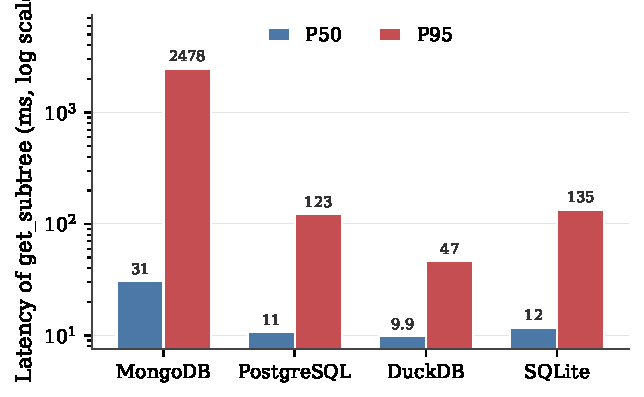
\includegraphics[width=0.6\linewidth]{figures/subtree.pdf}
\caption{\code{get\_subtree} latency on the large dataset (log scale). MongoDB is
measured on the deployed schema (covered structure scan,
Section~\ref{sec:solid}). The medians are within a small factor of each other;
MongoDB's tail is within ${\sim}1.4{\times}$ of PostgreSQL.}
\label{fig:subtree}
\end{figure}

\subsubsection{Write path}

On the write path (Table~\ref{tab:write}), PostgreSQL posts the lower update
latency of the two servers, but each \code{jsonb\_set} versions the row and leaves
a dead tuple for a later \code{VACUUM}. WiredTiger is MVCC too, yet it reclaims
obsolete document versions automatically, so an update-heavy workload carries no
growing bloat; its measured on-disk delta is small but noisy, since WiredTiger
reports storage in checkpoint-sized chunks. DuckDB is unsuitable for OLTP writes.

\begin{table}[h]
\caption{Write path (medium): 5{,}000 field updates, 2{,}000 incremental
inserts. ``Bloat'' is on-disk growth from the updates.}
\label{tab:write}
\begin{ctab}
\begin{tabular}{@{}lrrrr@{}}
\toprule
\hdr Engine & Upd.\ P50 & Upd.\ ops/s & Insert ops/s & Bloat \\
\midrule
\key MongoDB            & 0.242 & 4{,}050 & 5{,}586 & \best{0\,MB} \\
PostgreSQL (JSONB) & 0.123 & 7{,}856 & 8{,}732 & 7\,MB \\
DuckDB             & 2.966 & 332     & 450     & 7\,MB \\
SQLite             & \best{0.017} & \best{40{,}442} & \best{21{,}815} & \best{0\,MB} \\
\bottomrule
\end{tabular}
\end{ctab}
\end{table}

\subsubsection{Concurrency}

Single-call latency understates the server engines. Driving point lookups from a
growing pool of independent OS processes (no GIL bottleneck), both server engines
gain throughput with added clients, and the gap to the embedded engines narrows
far below what the single-call numbers suggest (Figure~\ref{fig:conc}). MongoDB
rises steadily across the whole range; PostgreSQL peaks near 16 clients; SQLite is
fastest in absolute terms but peaks earliest, within the first few clients, then
degrades as the processes contend on its single file. Repeated runs move the
peak positions and heights somewhat; the shapes hold.

\begin{figure}[h]
\centering
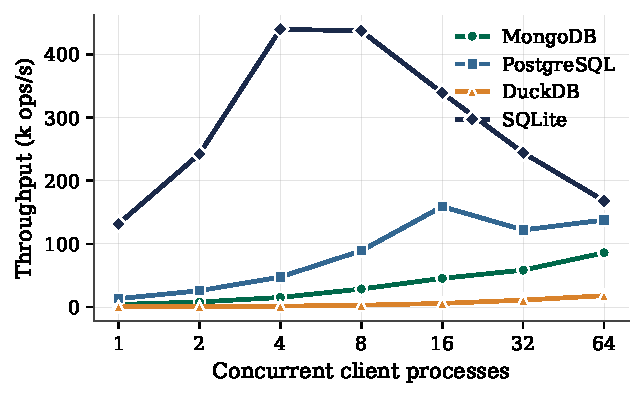
\includegraphics[width=0.6\linewidth]{figures/concurrency.pdf}
\caption{Point-lookup throughput versus concurrent client processes (medium).}
\label{fig:conc}
\end{figure}

\subsubsection{Multi-tenancy, batched reads, and deletion}

Mapping the retriever's calls to storage surfaces three operations the sections
above leave out: a per-query tenant filter when many trees share one store, the
batched id-list read the navigation step issues, and whole-tree deletion. We
measure them on the medium tree replicated into 25 co-resident trees
(1{,}771{,}075 rows in one store), with every read filtered by \code{tree\_id}
and served by a compound index led by \code{tree\_id}.

\paragraph{Multi-tenant selectivity.} With 25 trees in one collection, a
\code{tree\_id}-led index holds each read close to its single-tree latency
(Table~\ref{tab:mt}): the cost tracks index depth, not the number of co-resident
trees. MongoDB rises about $1.5{\times}$ on point and children lookups over the
single-tree medium figures (Table~\ref{tab:read}) for a $25{\times}$ larger
store, with no scan blow-up, and the MongoDB--PostgreSQL ordering is unchanged.

\begin{table}[h]
\caption{Per-query reads with 25 trees co-resident in one store, each filtered
by \code{tree\_id} (P50, ms).}
\label{tab:mt}
\begin{ctab}
\begin{tabular}{@{}lrrrr@{}}
\toprule
\hdr Operation & MongoDB & PostgreSQL & DuckDB & SQLite \\
\midrule
Point lookup    & 0.345 & 0.124 & 3.772 & \best{0.008} \\
Expand children & 0.372 & 0.147 & 3.073 & \best{0.014} \\
\bottomrule
\end{tabular}
\end{ctab}
\end{table}

\paragraph{Batched reads.} The navigation step returns a list of candidate node
ids, so the retriever fetches several nodes at once. One batched read
(\code{\$in} on MongoDB, \code{IN} on the relational engines) beats the
point-lookup loop it replaces on every engine, and the margin grows with batch
size because each iteration of the loop on a server engine is a round trip. At
200 ids MongoDB is 4.6\,ms batched against 273\,ms looped, a $60{\times}$ gap;
PostgreSQL is 1.4\,ms against 29\,ms (Table~\ref{tab:in}). MongoDB gains the most
because batching amortizes the per-call client overhead that costs it on single
reads; in-process SQLite, with no round trip, gains about $2{\times}$. The
retriever should resolve a candidate set with one batched read, not a loop.

\begin{table}[h]
\caption{Batched id-list read at 10, 50, and 200 ids against the 200-id
point-lookup loop it replaces (P50, ms per batch).}
\label{tab:in}
\begin{ctab}
\begin{tabular}{@{}lrrrr@{}}
\toprule
\hdr Engine & \multicolumn{3}{c}{Batched ($n$ ids)} & Loop \\
 & 10 & 50 & 200 & 200 \\
\midrule
MongoDB            & 0.46 & 1.56 & 4.56 & 273 \\
PostgreSQL (JSONB) & 0.27 & 0.78 & 1.40 & 29 \\
DuckDB             & 19.6 & 22.2 & 39.1 & 790 \\
SQLite             & \best{0.03} & \best{0.13} & \best{0.50} & \best{0.97} \\
\bottomrule
\end{tabular}
\end{ctab}
\end{table}

\paragraph{Deletion.} Removing a tree (one tenant, 70{,}843 of 1{,}771{,}075
rows) is a lifecycle operation, not part of retrieval. The delete is fast on
every engine, under four seconds, but none returns disk space on the delete
alone (Table~\ref{tab:del}). SQLite (\code{VACUUM}) and PostgreSQL
(\code{VACUUM FULL}) reclaim the removed tree's footprint through a full,
locking rewrite that takes 10 to 17\,s; MongoDB \code{compact} and DuckDB do not
measurably shrink the file for a single-tenant deletion, which is WiredTiger's
documented behavior of not returning space to the operating system on delete.
For MongoDB this mirrors the write path: WiredTiger carries no vacuum debt under
updates, and in exchange a one-off bulk delete does not auto-shrink. WiredTiger
reports \code{storageSize} in checkpoint-sized chunks, so changes below tens of
megabytes are reporting granularity, not reclaimed space.

\begin{table}[h]
\caption{Whole-tree delete and space reclamation (delete one of 25 trees).}
\label{tab:del}
\begin{ctab}
\begin{tabular}{@{}lrlrl@{}}
\toprule
\hdr Engine & Delete (rows/s) & Reclaim & Reclaim time & On-disk (before\,$\to$\,after) \\
\midrule
PostgreSQL (JSONB) & 157{,}578 & \code{VACUUM FULL} & 17.3\,s & 2.77\,$\to$\,2.66\,GB \\
SQLite             & 141{,}842 & \code{VACUUM}      & 10.6\,s & 2.56\,$\to$\,2.46\,GB \\
MongoDB            & 60{,}680  & \code{compact}     & 0.1\,s  & 911\,MB, no shrink \\
DuckDB             & 20{,}171  & checkpoint         & --      & 790\,MB, no shrink \\
\bottomrule
\end{tabular}
\end{ctab}
\end{table}

None of the three changes the benchmark conclusion: a \code{tree\_id}-led index
keeps tenant selectivity stable, batched reads remove the point-lookup loop cost,
and deletion behavior affects lifecycle maintenance rather than retrieval.

\subsection{MongoDB \code{get\_subtree} diagnosis}\label{sec:diagnosis}

MongoDB's unit of read is the whole document. A secondary index (here on
\code{path}) is a separate B-tree holding only the indexed field and a record
id; to return any other field, the engine must \emph{fetch} the full BSON
document and apply the projection to it. A point lookup is one such fetch and is
cheap. A subtree scan over monolithic node documents---structure, \code{title},
\code{summary}, and leaf \code{text} in one document---is tens of thousands of
them, each reading and decoding the whole document no matter how small the
projection. MongoDB's product team confirmed this read path when we raised it,
and confirmed that newer server versions do not change it (the 8.0 SBE
included). The data is resident and WiredTiger caches pages uncompressed, so the
cost is neither disk I/O nor decompression: it is per-document work---locate the
record, materialize the document, project, stream through the cursor---times
subtree size. The other retrieval operations touch few documents and stay fast
on any layout.

Two controlled measurements on the ten-million-node tree (one measuring client,
collection resident, the same 200 seeded subtree paths) narrow the cause. The
cost is not interference: the scan's latency barely moves while 16, 32, then 64
background processes hammer point lookups at the same server, with zero cache
evictions throughout. And it is not document size: splitting the wide
\code{text} field out removes ${\sim}75\%$ of every scanned document and leaves
subtree latency unchanged, and even ${\sim}150$-byte topology-only documents pay
most of the fetch cost. What gates the scan is the \emph{count} of fetches, so
only removing the fetch helps---which is what the deployed schema does
(Section~\ref{sec:solid}).

This is the trade-off of the document model, and it cuts both ways. A row store
materializes only the requested columns (PostgreSQL leaves the JSONB datum
compressed, since \code{node\_id} is its own column), and a column store reads
only the requested column, so both do far less per-node work on this one scan.
In exchange, storing a node's fields together is what makes every other
operation here cheap: point, children, and content reads, in-place field updates
(no vacuum debt), tenant-local sharding, and compact storage. The workload
matches the document model everywhere except the large-subtree scan---so the
deployed schema serves that one scan from an index instead.

\subsection{The deployed schema: decoupled structure and key-value
metadata}\label{sec:solid}

A node carries three kinds of data, and retrieval reads them on three different
paths, so the deployed schema stores them separately:

\begin{itemize}\itemsep2pt
\item \textbf{Structure} (\code{node\_id}, \code{path}, \code{parent\_id},
  \code{depth}): ${\sim}150$-byte topology documents carrying a lean
  \code{\{path,node\_id\}} covering index (\code{tree\_id}-led in production).
  Serves \code{get\_subtree} and navigation.
\item \textbf{Metadata} (\code{title}, \code{summary}): a key-value collection
  keyed by \code{\_id\,=\,node\_id}. Serves the nodes a view actually renders,
  by point read.
\item \textbf{Text}: leaf body text in its own collection keyed by node id.
  Serves \code{get\_entity} for the few nodes the model finally selects.
\end{itemize}

\begin{figure}[h]
\centering
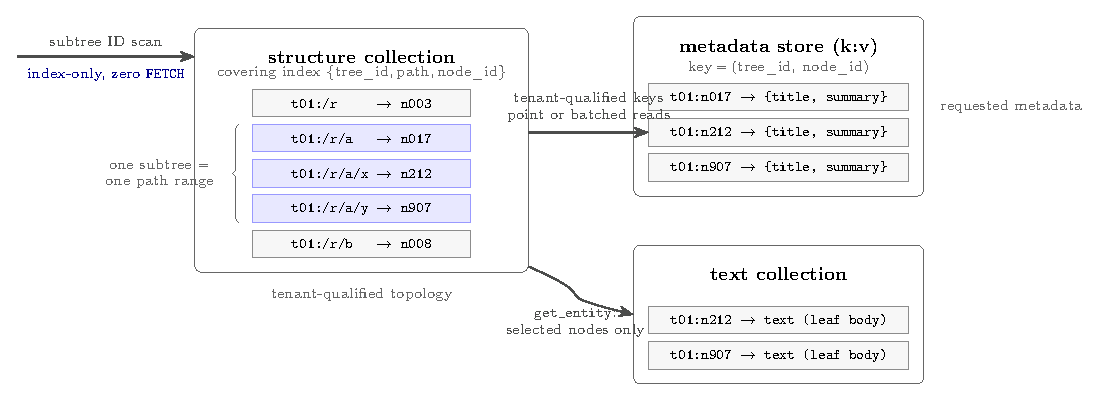
\includegraphics[width=0.92\linewidth]{figures/schema.pdf}
\caption{The deployed schema. A subtree is one contiguous range of the small
\code{\{path,node\_id\}} covering index, so \code{get\_subtree} never leaves the
index; the node ids it returns are the keys of the metadata store (k:v) and of
the text collection, each read only for the nodes actually rendered or
selected.}
\label{fig:schema}
\end{figure}

Under this layout (Figure~\ref{fig:schema}) the subtree scan never touches a
document: \code{explain}
confirms \code{PROJECTION\_COVERED} with \code{totalDocsExamined:\,0}, and
\code{get\_subtree} on the ten-million-node tree runs at $11.9$\,ms P50 /
$130$\,ms P95 (Table~\ref{tab:solid}), within ${\sim}1.4{\times}$ of PostgreSQL
at both percentiles (Table~\ref{tab:read}). The design has two traps, both
flagged by MongoDB's product team when we discussed it. Covered execution is
all-or-nothing: an index that serves the path filter but misses any projected
field, or a projection that keeps \code{\_id}, silently reinstates the
per-document \code{FETCH} (the structure scan without its covering index runs
${\sim}1.6{\times}$ slower even on ${\sim}150$-byte documents). And the covering
index's maintenance cost lands on writes, which the write-once tree turns into a
one-time ingest cost: bulk load first, build the index after.

\begin{table}[h]
\caption{\code{get\_subtree} on the deployed schema, 10M tree (one client, ms).
The covered structure scan is the hot path. The resolution rows price the worst
case: reading metadata for \emph{every} node of a ${\sim}36$k-node subtree in one
call.}
\label{tab:solid}
\begin{ctab}
\begin{tabular}{@{}p{6.6cm}rrl@{}}
\toprule
\hdr Read & P50 & P95 & Note \\
\midrule
\key Structure scan (covered, ids) & 11.9 & 130 & \code{totalDocsExamined:\,0} \\
Structure scan without covering index & 19.4 & 206 & \code{FETCH} per node \\
${+}$ metadata for all nodes, chunked \code{\$in} & 55.4 & 590 & ${\sim}36$ round trips \\
${+}$ metadata via server-side \code{\$lookup} & 381 & 4176 & one round trip \\
${+}$ metadata via \code{\$lookup}, clustered store & 279 & 3004 & one round trip \\
\bottomrule
\end{tabular}
\end{ctab}
\end{table}

The tree view does not render ${\sim}36$k titles at once; it renders a page of
nodes, and those resolve against the metadata store by \code{\_id} point reads at
sub-millisecond each (the point-lookup class of Table~\ref{tab:read}). Resolving
metadata for \emph{every} node of a large subtree in one shot is the worst case,
and it costs ${\sim}0.6$\,s at P95 via chunked \code{\$in}: a ${\sim}36$k-id \code{\$in}
overflows the 16\,MB command limit, so the client issues ${\sim}36$ chunked round
trips, and the metadata store performs ${\sim}36$k point lookups---the same
count-of-fetches mechanism as the monolithic scan, now confined to a path the
workload rarely takes. Two measured alternatives lose to it
(Table~\ref{tab:solid}). A server-side \code{\$lookup} from the structure scan
into the metadata store collapses the client round trips into one but performs
the same ${\sim}36$k per-id index probes inside the aggregation pipeline,
${\sim}7{\times}$ slower at both percentiles; a clustered metadata collection
(the record stored inside the \code{\_id} index) trims that by ${\sim}25\%$,
still far behind the chunked \code{\$in}. The clustered store must not,
however, be paired with the chunked \code{\$in} itself: with no separate
\code{\_id} B-tree, the planner turns each 1{,}000-id batch into a
\code{CLUSTERED\_IXSCAN} bounded only by the batch's min and max keys---observed
at ${\sim}7$M documents examined per batch on the 10M tree, an extrapolated
${>}100{\times}$ regression, so that measurement phase was aborted rather than
run to completion. If a deployment does need the full
\code{node\_id}+\code{title}+\code{summary} view from a single indexed query, the
alternative is to carry the metadata inside the covering index of a merged
collection: it stays covered and beats the monolithic scan, but the
multi-kilobyte \code{summary} key inflates that index to roughly the size of the
data itself, which is why the deployed schema keeps metadata in a key-value store
instead. Keep the anchored materialized-path range as the predicate either
way---an unanchored regex cannot form a range and must scan the whole index.

The split also keeps the hot working set small. For ten million nodes the
structure collection is $0.25$\,GB of data plus $0.56$\,GB of index on
disk---WiredTiger's prefix compression deduplicates the shared \code{path}
prefixes---and the metadata store adds $1.2$\,GB plus a $0.14$\,GB \code{\_id}
index: ${\sim}2.1$\,GB of navigation working set, against $5.2$\,GB for a
monolithic collection with \code{text} inline. At production scale, with many
trees or tenants sharing a host, that difference is what keeps the navigation
bytes cache-resident: body text never competes with structure for WiredTiger
cache.

\paragraph{Structural denormalization: the step beyond, unmeasured.} Nested Sets
or a tree-order \code{\_id} on a clustered collection turns the subtree into one
range query or a sequential read; a pre-computed subtree document turns it into a
point read. All are viable precisely because the tree is write-once (their cost
is paid once at ingest), and all would push the covered scan's remaining
${\sim}1.4{\times}$ toward parity. They were not measured in this pass; with the
deployed schema already at $168$\,ms P95 for an infrequent operation, the
remaining decision is whether the added schema complexity is justified.
(\code{\$graphLookup} is not a candidate---it re-traverses \code{parent\_id},
still materializes documents, and in 7.0 is capped at 100\,MB and ignores
\code{allowDiskUse}.)

\subsubsection{What a version bump or a license would not change}

The schema is the lever; neither an upgrade nor an edition change substitutes
for it. Across 8.0--8.3, the Express path accelerates point/equality lookups
only, block processing is scoped to time-series collections, and the
\code{\$graphLookup} disk-spill fix (SERVER-23980, in 8.2.0) helps only the
recursive alternative that loses to the range scan anyway---the
document-at-a-time \code{FETCH} is unchanged, as MongoDB's product team also
confirmed. On the Atlas side, the column-store index would read only projected
columns, but PageIndex never scans the whole corpus, and Search/Vector Search
serve relevance retrieval, not a range-projection scan. Every lever this
workload needs---schema, index, storage configuration---is on Community.

\section{Deployment optimization plan}\label{sec:opt}

The schema of Section~\ref{sec:solid} was measured on a cache-resident host. A
production deployment adds the opposite constraint: many trees or tenants can
make the working set larger than RAM, so the plan must also keep the hot
navigation data in cache. The deployment plan is therefore:

\begin{enumerate}\itemsep2pt
\item \textbf{Ship the decoupled schema.} Structure
  (\code{tree\_id}, \code{node\_id}, \code{parent\_id}, \code{depth},
  \code{path}) in the navigation collection; \code{title} and \code{summary} in
  a key-value metadata collection keyed by node id; body text in a third
  collection keyed by \code{(tree\_id,node\_id)}. This is what the covered
  subtree scan (Table~\ref{tab:solid}) is measured on, and at production scale
  it is also a cache-residency requirement: \code{get\_subtree} and navigation
  never need metadata or text bytes, and keeping them inline makes cold payload
  compete with hot structure for cache.
\item \textbf{Lead every index and shard key with \code{tree\_id}.} Multi-tenant
  reads must remain tenant-local: point lookup, children lookup, subtree range
  scan, and content fetch should all be served by compound indexes beginning with
  \code{tree\_id}. This preserves selectivity as the number of trees grows and is
  the natural shard key for horizontal scale.
\item \textbf{Keep the covering index lean and exactly aligned with the
  projection.} A \code{\{tree\_id,path,node\_id\}} index serves subtree scans
  index-only; build it after bulk load so its maintenance cost is paid once.
  Covered execution is all-or-nothing---a missing projected field, or \code{\_id}
  left in the projection, silently brings the per-document \code{FETCH} back---so
  treat \code{explain} showing \code{totalDocsExamined:\,0} as a deployment
  check, not a one-time observation. Do not put the multi-kilobyte \code{summary}
  into the covering key: the metadata store already serves it by point read, and
  carrying it in the index costs index bytes comparable to the data itself.
\item \textbf{Denormalize hot subtree views only after measuring demand.} If
  \code{get\_subtree} remains a top latency contributor, use write-once structure
  to precompute bounded structure+summary subtree views, or add Nested Sets /
  tree-order \code{\_id} for range-locality. These remove even the covered scan's
  per-key work, but they add storage amplification and more complicated ingest.
\end{enumerate}

\noindent The rollout test should reproduce the missing production condition:
run the decoupled schema against a monolithic inline-text layout with the
WiredTiger cache sized below the inline layout's working set and above the
decoupled navigation working set. That experiment prices the cache-residency
benefit directly; this benchmark cannot, because every layout it measured was
already cache-resident.

\section{Conclusion}

The benchmark supports MongoDB for the PageIndex retrieval workload. Point
reads, children reads, content fetches, writes, multi-tenant selectivity,
batched reads, concurrency, and footprint are all acceptable or favorable, and
the one operation that stresses the document model---\code{get\_subtree}, a
range scan matching tens of thousands of nodes---is a schema problem with a
measured solution, not an engine ceiling. Served from the deployed schema's
structure collection by a covering index, it runs with zero document fetches at
$11.9$\,ms P50 / $130$\,ms P95 on the ten-million-node tree, within
${\sim}1.4{\times}$ of PostgreSQL at both percentiles.

The diagnosis behind that design is mechanical and vendor-confirmed: MongoDB
reads whole documents, so a non-covered scan pays per matched document
regardless of projection, and neither newer server versions nor cache sizing
changes it. Decoupling puts on the scan's path only the bytes the scan needs
(structure under a covering index) and serves everything else by the reads the
document model is good at (key-value point lookups for metadata, content
fetches for selected text). The remaining validation is deployment-shaped, not
mechanism-shaped: the cache-constrained A/B that prices the split's residency
benefit, and the structural denormalizations (Nested Sets, tree-order
\code{\_id}, precomputed subtree views) if a measured workload ever needs the
last ${\sim}1.4{\times}$.

\end{document}
